%\begin{flushleft}


\chapter{\large PROJECT PLANNING AND MANAGEMENT}

\section{\normalsize PROJECT DEVELOPMENT LIFECYCLE}
\justifying
\begin{center}
\begin{figure}[hbtp]
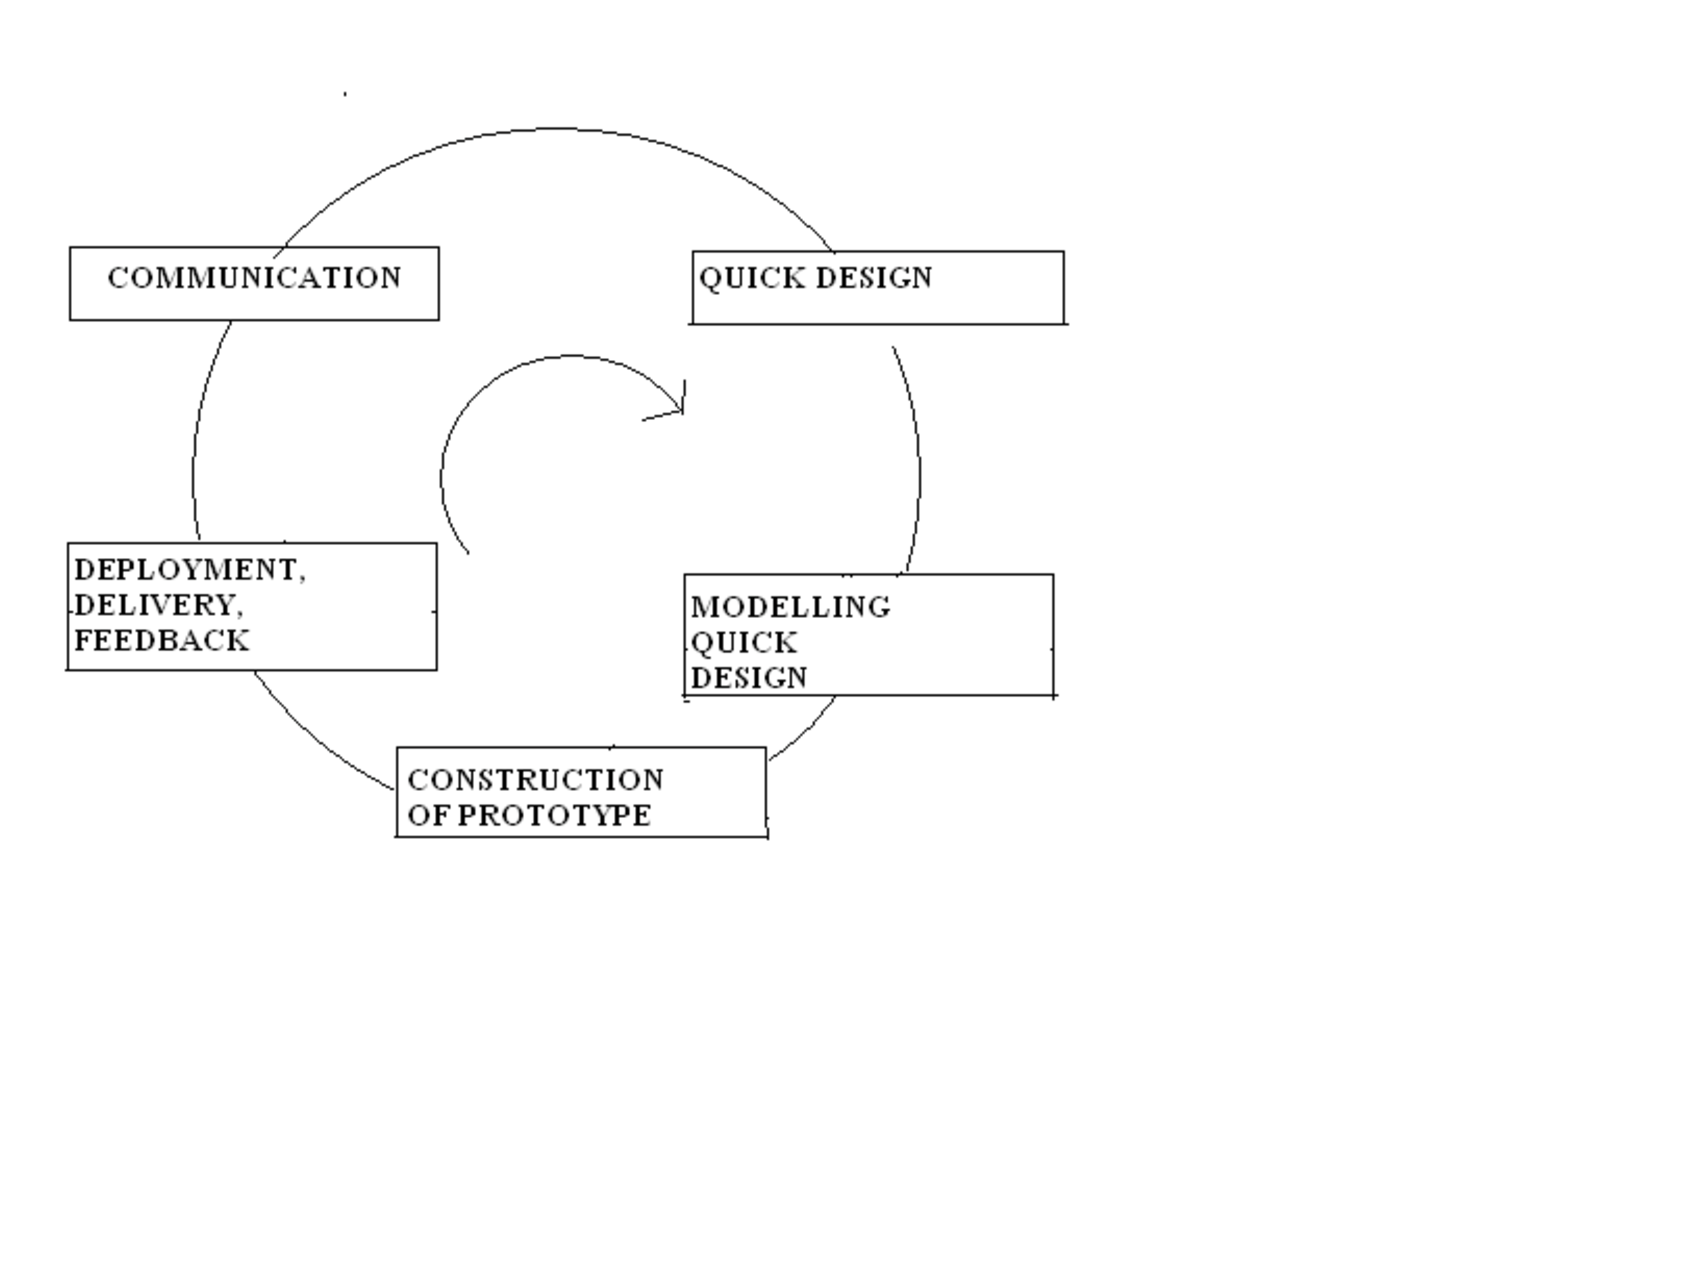
\includegraphics[width=20cm,height=13cm]{pdl.eps}
\caption{Project Devlopment Life Cycle}
\end{figure}
\end{center}
\newpage
\textbf{1. Requirement Gathering:}\\
\hspace*{1cm}The project development lifecycle starts with understanding all the requirements of the system. It involves the communication between the user and the developer. Based upon the functionalities of the system and the points stated by the end user the requirements of the project are decided. It also involves generating the Software Requirement Specification (SRS).\\
Requirement of project is – \\
\hspace*{1cm}1.	Flatgraph with numbered nodes, weight\\
\hspace*{1cm}2.	Database that stores the flatgraph, partition and supergraph\\
\hspace*{1cm}3.	GUI that makes path viewing easier\\
\hspace*{1cm}4.	Authentication of user for security\\
\hspace*{1cm}5.	Platform Independent language to be used for coding
\vspace{.2in}\\
\textbf{2.Planning:}\\
\hspace{1cm}The planning phase includes complete estimation and scheduling of the activities to be performed in the project. It includes the distribution of work, the estimated time to complete the project, the estimated cost, job scheduling and tracking.\\
\hspace{1cm}
Information gathering, study of IEEE papers and estimation of resources required is completed before beginning of documentation and designing.\\
\hspace{1cm}
After completion of documentation and design project work will be evenly distributed in team. Team will first study the project flow. Database being less complex will be designed precisely by one team member. Then another team member will work on the gui design. The other two members will begin with coding part. All these sections have to start simultaneously.\\
\hspace{1cm}
Project will be divided roughly into 3 phases. Phase 1 has to be completed till mid December. Phase 2 has to be completed till January end and Phase 3 has to be completed till February end.
\vspace{.2in}\\
\textbf{3.Modeling and Design:}\\
\hspace*{1cm}It includes detail requirement analysis and project design. It also involves development of  algorithms and various architectural concepts like use case diagrams, flowcharts  etc.\\
\hspace*{1cm}
Use Case Diagram, Class Diagram, DFD, ERD, Activity Diagram, Sequence Diagram and State Transition Diagram are designed before 2nd Review. Complete detailing and flow of project is demonstrated by these diagrams.\\

\textbf{Project is divided in 3 phases –}\\
\hspace*{1cm}\textbf{Phase 1-}\\
\hspace*{1cm}
Algorithms will be thoroughly studied before beginning of database design. Flatgraph will be designed and module will be designed to encode the flatgraph. The encoded flatgraph will be stored in database.\\
\hspace*{1cm}
Gui will be developed. Authentication for system security will be designed.\\
\hspace*{1cm}\textbf{Phase 2-}\\
\hspace*{1cm}
After encoding the flatgraph into database coding for partition and supergraph must begin. Database design for storing partition and supergraph will be done. \\
\hspace*{1cm}
Gui for creating, encoding partition and supergraph will be designed simultaneously.\\
\hspace*{1cm}\textbf{Phase 3-}\\
\hspace*{1cm}
During coding of path retrieval normalization of database and perfection of gui will be carried out.
Development of Path Retrieval module will be time consuming thus in this phase focus will be mainly on path retrieval module.
\vspace{.2in}\\
\textbf{4.Construction:}\\
It includes coding and testing steps:\\
\hspace*{1cm}
1.	Coding: Design details are implemented using appropriate programming language.\\
\hspace*{1cm}
2.	Testing: Testing is carried out to check whether flow of coding is correct and to point out the errors of the program.\\
Coding will be done in following steps –\\
\hspace*{1cm}
1.	Encoding flatgraph\\
\hspace*{1cm}
2.	Authentication of user\\
\hspace*{1cm}
3.	Create and encode partition\\
\hspace*{1cm}
4.	Develop gui for the same\\
\hspace*{1cm}
5.	Create and encode supergraph\\
\hspace*{1cm}
6.	Develop gui for the same\\
\hspace*{1cm}
7.	Develop path retrieval module\\
\hspace*{1cm}
8.	Develop gui for usage of customer\\

Testing will be done with overall gui and algorithms. Testing will be performed timely and before deployment of project.
\vspace{.2in}\\
\textbf{5.Deployment:}\\
	\hspace*{1cm}It includes software delivery , support and feedback from user. If the user suggests some corrections, or demands additional capabilities then changes are required for such corrections or enhancements.  \\
\hspace*{1cm}
	Deployment will be done after complete testing of the project.\\


\section{\normalsize PROJECT DELIVERABLES}


Deliverables for our project will include:\\
1.\textbf{Project report}\\
\hspace*{1cm}It includes Software Requirement Specification, All design details, technical diagrams, schedule, cost, testing details etc..\\
2.\textbf{CD}\\
\hspace*{1cm}It contains the Hierarchical Optimization Of Optimal Path Finding System GUI set up.\\
3.\textbf{Manual}\\
\hspace*{1cm}Provides all procedures required while using the system. Also contains the Help.
\\

\section{\normalsize TASKS AND MILESTONES}
\subsection{Tasks}
\textbf{The following tasks have to be performed:}\\
\hspace*{1cm}1.	Database with tables required for flat-graph, partitions and supergraph will be created.\\
\hspace*{1cm}2.	Authentication mechanism will be developed.\\
\hspace*{1.5cm}Admin only is allowed to create, encode partitions and supergraph.\\
\hspace*{1cm}3.	Modules to create and encode partitions and supergraph will be developed.\\
\hspace*{1cm}4.	Optimal Path Retrieving module will be developed.\\

\subsection{Milestones}
	\hspace*{1cm}In general the following major milestones can be considered "completed"� when the criteria noted have been met.\\
	
1)  Development of different modules:
   It is necessary to divide the project in different modules and work on those modules individually.
 
2)	Testing of modules individually:
 The modules which are developed are then tested one at a time. All the elements related to a module are tested and if needed modification is done at that time.
 
 3)	 Module Integration :
    After all the modules are tested individually they are combined to form the whole project.

4)	Testing Project as a Whole :
    After integrating the modules the project is tested as a whole to see if any bugs are left. They are rectified then and the project is then ready for Deployment.


5)	Follow up of Guidelines :
    It is seen that all Guidelines given are maintained and all the expectations of the user from the application are fulfilled. Also the application should be user friendly.

\vspace{.2in}
\textbf{Hierarchical Optimization of Optimal Path Finding System will have following}\\
\vspace*{0cm}\textbf{milestones:}\\
\hspace*{1cm}1.	Authentication of Admin\\
\hspace*{1cm}2.	Creation and encoding of Partitions from flatgraph\\
\hspace*{1cm}3.	Creation and encoding of Supergraph from partitions\\
\hspace*{1cm}4.	Maintenance of Hierarchical Encoded Path View(HEPV)\\
\hspace*{1cm}5.	Optimal Path Retrival using Hierarchical Encoded Path View(HEPV)\\

\section{\normalsize COST AND EFFORT ESTIMATION}
\hspace{1cm}The constructive Cost Model is generally used for estimation measure of project cost, project duration, manpower etc.\\
\hspace*{1cm}Like all estimation models, the COCOMO model requires sizing information .This information can be specified in terms of:
\begin{description}
\item[\hspace*{1cm}$\bullet$]Object Point(OP)
\item[\hspace*{1cm}$\bullet$]Function Point(FP)
 \item[ \hspace*{1cm}$\bullet$]Lines Of Source Code(KLOC)
  \end{description}
For our project we use sizing information in the form of line of source code(KLOC).
\begin{description}
\item[\hspace*{1cm}$\bullet$]Total lines of code for our Project,KLOC = 3.6k(approx)
\item[\hspace*{1cm}$\bullet$]Cost of each person per month Cp = Rs.1500/-(approx)
\end{description}

\textbf{Efforts} \\
\hspace*{1cm}Equation for calculation of efforts in person-months for COCOMO model is:\\
\hspace*{3.5cm} E = a*(KLOC)$^{b}$\\
\hspace*{1cm}Where,\\
 \hspace*{1.5cm}a=3.0\\
  \hspace*{1.5cm}b=1.12\\
   \hspace*{1.5cm}E=Efforts in person-months\\
\hspace*{3.5cm}E=3.0*(3.6)$^{1.12}$\\
\hspace*{3.5cm}E=12.59 person-months\\
\hspace*{1cm}Total efforts of 12.59 person-months are required to complete the project successfully\\

\textbf{Duration of Project:}\\ 
\hspace*{1cm}Equation for calculation of Duration of projects in months for COCOMO model is:\\
\hspace*{3.5cm} D = A * (E)$^{b}$ \\
 \hspace*{1cm}Where,\\
\hspace*{1.5cm}a=2.5\\
\hspace*{1.5cm}b=0.32\\
\hspace*{1.5cm}D=Duration of Project in months.\\
\hspace*{3.5cm}D=2.5*(12.59)$^{0.32}$ \\

\hspace*{1cm}The approximate duration of project is 5.63 months\\

\textbf{Number of team members:}\\
 \hspace*{1cm}The equation for calculation of Number of team members required for completion of project, using COCOMO model is:\\
\hspace*{3.5cm}N = E / D\\

\hspace*{1cm}Where,\\
 \hspace*{1.5cm}N=number of team members required.\\
 \hspace*{1.5cm}E=Efforts in person-months.\\
  \hspace*{1.5cm}D=Duration of project in months.\\
 \hspace*{3.5cm}N=12.59/5.63\\
 \hspace*{3.5cm}N=3  (approx)\\

\textbf{Cost of project:}\\
 \hspace*{1cm}Equation for calculation of cost of project, using COCOMO model is:\\
\hspace*{3.5cm} C = D * Cp\\
	
\hspace*{1cm} Where,\\
\hspace*{1.5cm}	C=Cost of Project.\\
 \hspace*{1.5cm} D=Duration of Project in Months.\\
 \hspace*{1.5cm}Cp=Cost incurred per person-month\\
\hspace*{3.5cm}C=5.63 * 6400\\

\hspace*{1.5cm}Therefore total cost of project is Rs. 36032 /-(approx)\\

		 

\section{\normalsize RISKS}
\subsection{Technical Risks:}
\hspace*{1cm}No technical risks as such is existing since the Operating System being used is Windows, which is well established as well as accepted. Maintenance problem could exist in system.
\subsection{Product Size Risks:}
\hspace*{1cm}The size estimate in LOC of our project may be significantly low. This may affect the schedule as well as upset the estimate and total cost of our project. 

\subsection{Business Risks:}
\hspace{1cm}The top five business risks are \\
\hspace*{1cm}1)	Building an excellent product or system that nobody really wants (market risk).\\
\hspace*{1cm}2)	Building a product that no longer fits into the overall business strategy for the company (strategy risk).
\\ \hspace*{1cm}3)	Building a project that the sales force does not understand how to sell.
\\ \hspace*{1cm}4)	Losing the support of senior management due to a change in focus or change in people (management risk).
\\ \hspace*{1cm}5)	Losing budgetary or personnel commitment (budget risk).

\subsection{System Failure}
\hspace*{1cm}If Database crash during the path retrieval then it is tedius task to recover the database. 

%\end{flushleft}